\documentclass[DM,lsstdraft, authoryear,toc]{lsstdoc}
% lsstdoc documentation: https://lsst-texmf.lsst.io/lsstdoc.html
\input{meta}

% Package imports go here.
\usepackage{amsmath}
\usepackage{amssymb}
% Local commands go here.
\newcommand{\rmd}{\mathrm{d}^2}
%If you want glossaries
%\input{aglossary.tex}
%\makeglossaries

\title{Consistent galaxy colors with \\ Gaussian-Aperture and PSF photometry}

% Optional subtitle
% \setDocSubtitle{A subtitle}

\author{%
Arun Kannawadi
}

\setDocRef{DMTN-190}
\setDocUpstreamLocation{\url{https://github.com/lsst-dm/dmtn-190}}

\date{\vcsDate}

% Optional: name of the document's curator
% \setDocCurator{The Curator of this Document}

\setDocAbstract{%
Gaussian-Aperture and PSF photometry algorithm measures consistent colors for extended sources such as galaxies that are largely independent of seeing.
This technote briefly presents the mathematical description of the algorithm and focuses on its implementation in the Rubin Science Pipelines.
This document also serves as a reference for several of the analytical calculations that are tested in the unit tests.
}

% Change history defined here.
% Order: oldest first.
% Fields: VERSION, DATE, DESCRIPTION, OWNER NAME.
% See LPM-51 for version number policy.
\setDocChangeRecord{%
  \addtohist{1}{YYYY-MM-DD}{Unreleased.}{Arun Kannawadi}
}


\begin{document}

% Create the title page.
\maketitle
% Frequently for a technote we do not want a title page  uncomment this to remove the title page and changelog.
% use \mkshorttitle to remove the extra pages

% ADD CONTENT HERE
% You can also use the \input command to include several content files.
\section{Introduction}
Galaxy photometry is a hard problem, if not impossible.
Unlike stellar photometry (in non-crowded regions) where we know the true, intrinsic profile (a point source), we do not usually know the profile for extended sources (galaxies).
This is especially true at the outskirts of the galaxies where they smoothly blend in with the sky background and we need to model the wings of the PSFs accurately.
Errors in either of these models lead to systematic errors.
%Aperture correction is not immune to this as it requires making an assumption about the tail of the galaxies.
%Total fluxes are model-dependent (and observation dependent) and are ill-defined in practice.

Fortunately, having total fluxes is sufficient, and not necessary, to define colors of objects.
It is often easier to obtain color information from multiband images, and is sufficient for obtaining scientifically interesting quantities such as photometric redshifts.
Total flux or magnitudes is useful to quantify stellar luminosities (SED of total light emitted in all the bands) and masses.
However, in addition to a total magnitude in a reference band, ratios of fluxes in different bands (colors) are sufficient for studies involved in photometric redshifts, stellar populations, star-formation rates etc.
They usually have different requirements, and will coincide for unresolved/point sources.

\subsection{Notation}
Throughout this technote, we use the following notation consistently.

\begin{itemize}
    \item $g({\bf x})$: unobservable pre-seeing galaxy profile
    \item $G({\bf x})$: observable image of galaxy with a Gaussian PSF
    \item $I({\bf x})$: observed image of the galaxy with some PSF
    \item $P({\bf x})$: PSF profile in the observed image $I({\bf x})$, including the pixel response.
    \item $K({\bf x})$: convolution kernel that converts $I({\bf x})$ to $G({\bf x})$, with a desired Gaussian PSF.
    \item $w({\bf x})$: aperture applied on the pre-seeing image $g({\bf x})$ (referred to as `pre-seeing aperture')
    \item $A({\bf x})$: aperture applied on the observed image $I({\bf x})$ (referred to as `post-seeing aperture')
\end{itemize}

\subsection{Consistent colors}
\textbf{Definition:} If we apply the same weight to each star in a galaxy across all bands, then it is a consistent color.
In practice, this means use the same weight function $w({\bf x})$ across all bands.
If the galaxy has the same morphology in two bands, then a consistent color is the same as 'complete' color,
which is the ratio of total fluxes.

If we model a galaxy purely as a collection of stars, $g^{(b)}({\bf x}) = \sum_* f^{(b)}_*\delta_D({\bf x}-{\bf x}_*)$.
Its total flux $F^{(b)} = \int\rmd{\bf x}\, g^{(b)}({\bf x}) = \sum_* f^{b}_*$.
We define \emph{complete color} (or total color) as the color of a galaxy obtained from its total fluxes.
Given two passbands $b_1$ and $b_2$, a \emph{complete color} is defined as
\begin{equation}
  C(b_1,b_2) \equiv \frac{F^{(b_1)}_w}{F^{(b_2)}_w} = \frac{\int\rmd{\bf x}\, g^{(b_1)}({\bf x})}{\int\rmd{\bf x}\, g^{(b_2)}({\bf x})}
\end{equation}
It is worth noting that a complete color is not the same as the average color of its constituent stars, i.e.,
$C(b_1,b_2) \ne \left\langle \frac{f^{(b_1)}_*}{f^{(b_2)}_*} \right\rangle_*$

Given two passbands $b_1$ and $b_2$, a \emph{consistent color} is defined as
\begin{equation}
  C_w(b_1, b_2) \equiv \frac{F^{(b_1)}_w}{F^{(b_2)}_w} = \frac{\int\rmd{\bf x}\,w({\bf x}) g^{(b_1)}({\bf x})}{\int\rmd{\bf x}\,w({\bf x}) g^{(b_1)}({\bf x})}
\end{equation}

A complete color is a consistent color, as it corresponds to the choice of $w({\bf x}) \equiv 1$.
A consistent color defined with some weight $w$ is insensitive to $w$ and identical to complete color in the absence of color gradients.
While $F^{(b)}_w$ is not an estimator of \emph{total} flux, the ratio ${F^{(b_1)}_w}/{F^{(b_2)}_w}$ (consistent color) matches the ratio of total fluxes ${F^{(b_1)}}/{F^{(b_2)}}$ (complete color)
if the morphology is the same in the two bands, i.e., $g^{(b)}({\bf x}) \propto F^{(b)} g({\bf x})$ for $b=b_1,b_2$.
While this is generally not true for galaxies, it is true for stars and other point sources.
In fact, $F^{(b)}_w = F^{(b)}$ for point sources if $w({\bf x})$ is normalized to have a unit amplitude.
For extended sources, $C_w(b_1, b_2)$ is sensitive to the
weight function. This means that in the presence of a non-trivial weight $w({\bf x})$, galaxy color is not invariant to moving the stars around within the galaxy, which the ratio of total fluxes is insensitive to. The complete color is only sensitive to changes in the fraction of different stellar populations within a galaxy.

Having a compact weight function allows extracting the color information from the bright regions of a galaxy by upweighting the central regions.
If the color gradients were absent, one could choose the formally optimal (or a near-optimal) weight function $w({\bf x})$ for each galaxy to maximize the signal-to-noise ratio of its color estimate.
However, since the color of a galaxy is sensitive to $w$ in practice, varying $w$ for each galaxy may lead to difficulty in calibrating photometric redshift codes.
Furthermore, choosing the shape\footnote{It is unavoidable to use the detection peaks from the same image.} of $w$ from the same image we measure the flux from can lead to the estimate being non-linear and biased.
It might be preferable to use a weight function that is circular and slightly sub-optimal that is appropriate to a population of galaxy.
Having a variety of weight functions allows one to study the population of stars as a function of radial distance.

\begin{comment}
\subsection{Noise bias}
Ideally, we want linear estimator.
This is impossible if the weight function is centered based on the measured centroid from the same image.
Adaptive the shape of the weight function to match the observed shape of the source worsens it.
However, if even the flux estimator is linear, the estimator for color as the ratio of flux estimators is biased, as it is not linear.
Morever, the bias depends on the color in the non-trivial way.
It would be beneficial to use adaptive weight function to perform optimal photometry instead of circular apertures with pre-defined widths.
We provide both the
\end{comment}
\section{Gaussian Aperture and PSF photometry}

GAaP is essentially an aperture photometry algorithm that adjusts the aperture depending on the seeing, such that the "flux" measured is seeing-independent for a wide range of seeing.
Intuitively, if the PSF is large, then one needs to use a smaller aperture and vice versa.
We derive this formalsm mathematically below.

\subsection{Formalism}
The flux $F_A$ of a galaxy image $I({\bf x})$ with an aperture function $A({\bf x})$ is defined as
\begin{align}
  F_A &:= \int\rmd{\bf x}\, A({\bf x}) I({\bf x}) \\
      &= \int\rmd{\bf x}\, A({\bf x}) \int\rmd{\bf y}\,g({\bf y}) P({\bf x}-{\bf y}) \\
      &= \int\rmd{\bf x}\int\rmd{\bf y}\, A({\bf x}) g({\bf y}) P({\bf x}-{\bf y}) \\
      &= \int\rmd{\bf y} \left(\int{\rmd}{\bf x}\, A({\bf x})P^*({\bf y}-{\bf x}) \right) g({\bf y}),
\end{align}
where in the last step, we swapped the order of integration in the last equation and defined a flipped PSF $P^*$ such that $P^*({\bf r}) = P(-{\bf r})$.

The pre-seeing aperture $w({\bf y})$ is related to the post-seeing aperture $A({\bf x})$ via the
flipped PSF $P^*$.
\begin{equation}
  w({\bf y}) := \int{\rmd}{\bf x}\, A({\bf x})P^*({\bf y}-{\bf x})
\end{equation}
Thus, if the post-seeing aperture $A$ is adjusted for seeing such as the pre-seeing aperture remains the same for all bands,
then the fluxes estimated with $w$ result in consistent colors. Given the choice of the intrisic weight function (pre-seeing aperture) $w({\bf x})$, the post-seeing aperture used for photometring the source is formally given as
\begin{equation}
  A({\bf x}) = \left(w \otimes^{-1} P^*\right)({\bf x}),
\end{equation}
where $\otimes^{-1}$ denotes deconvolution operator.
Thus, the use of this post-seeing aperture for photometring the source is designed to give colors that are insensitive to the seeing (DMS-REQ-0276).

In GAaP algorithm, the pre-seeing aperture is chosen to be a Gaussian function $w({\bf x}) = \exp\left(-\frac{1}{2}{\bf x}^T W_\text{int}^{-1}{\bf x}\right)$ for some $2\times 2$ positive-definite
\footnote{A $2\times 2$ positive-definite matrix $M$ is a symmetric matrix with real entitites if and only if ${\bf x}^T M {\bf x} > 0$ for all ${\bf x} \in \mathbb{R}^2$. In practice, this implies $M_{11} >0$, $M_{22}>0$ and $\det(M)>0$.}
matrix $W_\text{int}$.
The choice of a Gaussian function over a flat top-hat aperture allows one to obtain colors from the bright central region of the galaxy well above the sky background and gives vanishingly low weight to the tail that is hidden in the noise.
Furthermore, in addition to the SNR argument, the central parts of the galaxies are redder in color as they contain older population of stars.
These populations are relatively easier\footnote{\tiny\url{https://project.lsst.org/meetings/law/sites/lsst.org.meetings.law/files/Galaxy\%20Photometry\%20-\%20Konrad\%20Kuijken.pdf}} to obtain photometric redshifts from, thereby increasing the fidelity of the photo-z measurements.

Rather than using the formal solution to find the post-seeing aperture, the implementation of the algorithm uses a two-step procedure:
\begin{enumerate}
  \item Convolve the image $I({\bf x})$ by a kernel function $K$ to obtain an PSF-Gaussianized image $G({\bf x})$ which has a circular Gaussian PSF of size $p$
  \item Photometer the resulting image using the $A({\bf x}) = \exp\left(-\frac{1}{2}{\bf x}^T(W_\text{int}-p^2\mathbf{1})^{-1}{\bf x} \right)$, where $W_\text{int}-p^2\mathbf{1}$ is positive-definite.
\end{enumerate}

Hence, the algorithm is named Gaussian-Aperture and (Gaussian) PSF.

Based on Eq. A16 of \cite{Kuijken2015}, the GAaP flux with an aperture parameter ${\bf W}$ is defined as follows:
\begin{align}
  F_{\bf W} &\equiv \int\rmd{\bf x}\, g({\bf x})\exp\left( -\frac{1}{2}{\bf x}^T{\bf W}^{-1}{\bf x} \right) \\
        &= \frac{1}{2}\frac{\det({\bf W})^{1/2}}{\det({\bf W}-p^2{\bf 1})^{1/2}}\times 2\int\rmd{\bf x} G(\bf x) \exp\left(-\frac{1}{2}{\bf x}^T({\bf W}-p^2{\bf 1})^{-1}{\bf x}\right),
  \label{eq:A16}
\end{align}
where $G({\bf x})$ is the image of $g({\bf x})$ after convolution by a Gaussian PSF of size $p$.
Given a set of passbands $\{b_1, b_2, \dots b_n \}$, the corresponding $F_{\bf W}$s can be used to obtain any of the $(n-1)$ independent color terms.

In the limit $g({\bf x}) \rightarrow F\delta({\bf x})$, the GAaP flux $F_{\bf W}$ equals $F$.
The fact that GAaP fluxes are estimates of total fluxes for point sources is a useful one in practice.
This enables the use the standard photometric calibrations developed for other flux measurement algorithms usable for GAaP as well.

\section{Implementation in the Rubin science pipelines}
GAaP algorithm is implemented as a measurement plugin that can be run in forced mode.

\subsection{Definitions}
This subsection consists the definition of various configuration parameters, internal variables and flags that may be needed to use the algorithm effectively.

The size $p$ is set as some factor $f$ times the trace radius of the original PSF for a given source in a given band.
The scaling factor $f$ is enforced to be larger than unity to avoid deconvolution.
The scaling factors can be configured using the \texttt{scalingFactors} field.
By default, $f=[1.15]$.

We use the basic building blocks in \texttt{modelPsfMatchTask} to Gaussianize the PSF, with one key difference:
by default we convolve the PSF-matching kernel in Fourier space to speed up the computation (this may be configured to carry out the convolution in real-space or overlap-add method if preferred).
Occasionally, the solution for the kernel fails, and no measurement is possible for any values of $W_\text{int}$.
We mark such failures by setting \texttt{\_flag\_gaussianization}.

The factor multiplying the integral, especially $\det({\bf W}-p^2{\bf 1})^{1/2}$, is required to keep $F_{\bf W}$ PSF-independent.
Internally, we refer to this factor, the square root of the ratio of determinants, as \texttt{fluxScaling}.
We scale the \texttt{instFlux} value from the \texttt{computeFixedMomentsFlux} method with \texttt{fluxScaling}.

The simplest case of apertures are those described by pre-determined circular apertures ${\bf W}_\text{int} = \sigma_w^2\mathbf{1}$ for some $\sigma_w$.
The set of $\sigma_w$ is configurable using \texttt{sigmas} parameter.
For such circular apertures, $\texttt{fluxScaling} = \frac{1}{2}\frac{\sigma_w^2}{\sigma_w^2-p^2}$,
where ${\bf W} = \sigma_w^2 \bf{1}$.
A necessary condition for the measurement to be valid is that $\sigma_w$ must be larger than $p$.
When this condition is not met, usually for bad seeing images, \texttt{\_flag\_bigPsf} is set for the corresponding measurement.

Additionally, we also use one elliptical aperture that is adapted to the galaxy.
We adopt the following heuristic to increase the signal-to-noise ratio:
The post-seeing aperture is chosen to be the adaptive moments of the source in the reference band.
For the purpose of optimal photometry alone, we assume that the PSF in the reference band is Gaussian and add the PSF adaptive moments to the source adaptive moments to obtain $W_\text{int}$.
The intrinsic aperture $W_\text{int}$ is then used in all measurement bands.
This simple heuristic gives us a near-optimal photometry.
This differs from true optimal aperture depending on how non-Gaussian the PSF is.
However, given the low sensitivity to the aperture parameters, the heuristic aperture leads to an increase in SNR,
with the improvement being larger for galaxies with larger ellipticity values.
% For the purpose of finding the optimal (elliptical) aperture, we assume that the PSF is Gaussian described by its PSF shape.
% We set ${\bf W} - {\bf W}_\text{psf}$ to match the observed shape for the galaxies.

\subsection{Evaluating the integrals}
\begin{figure}
    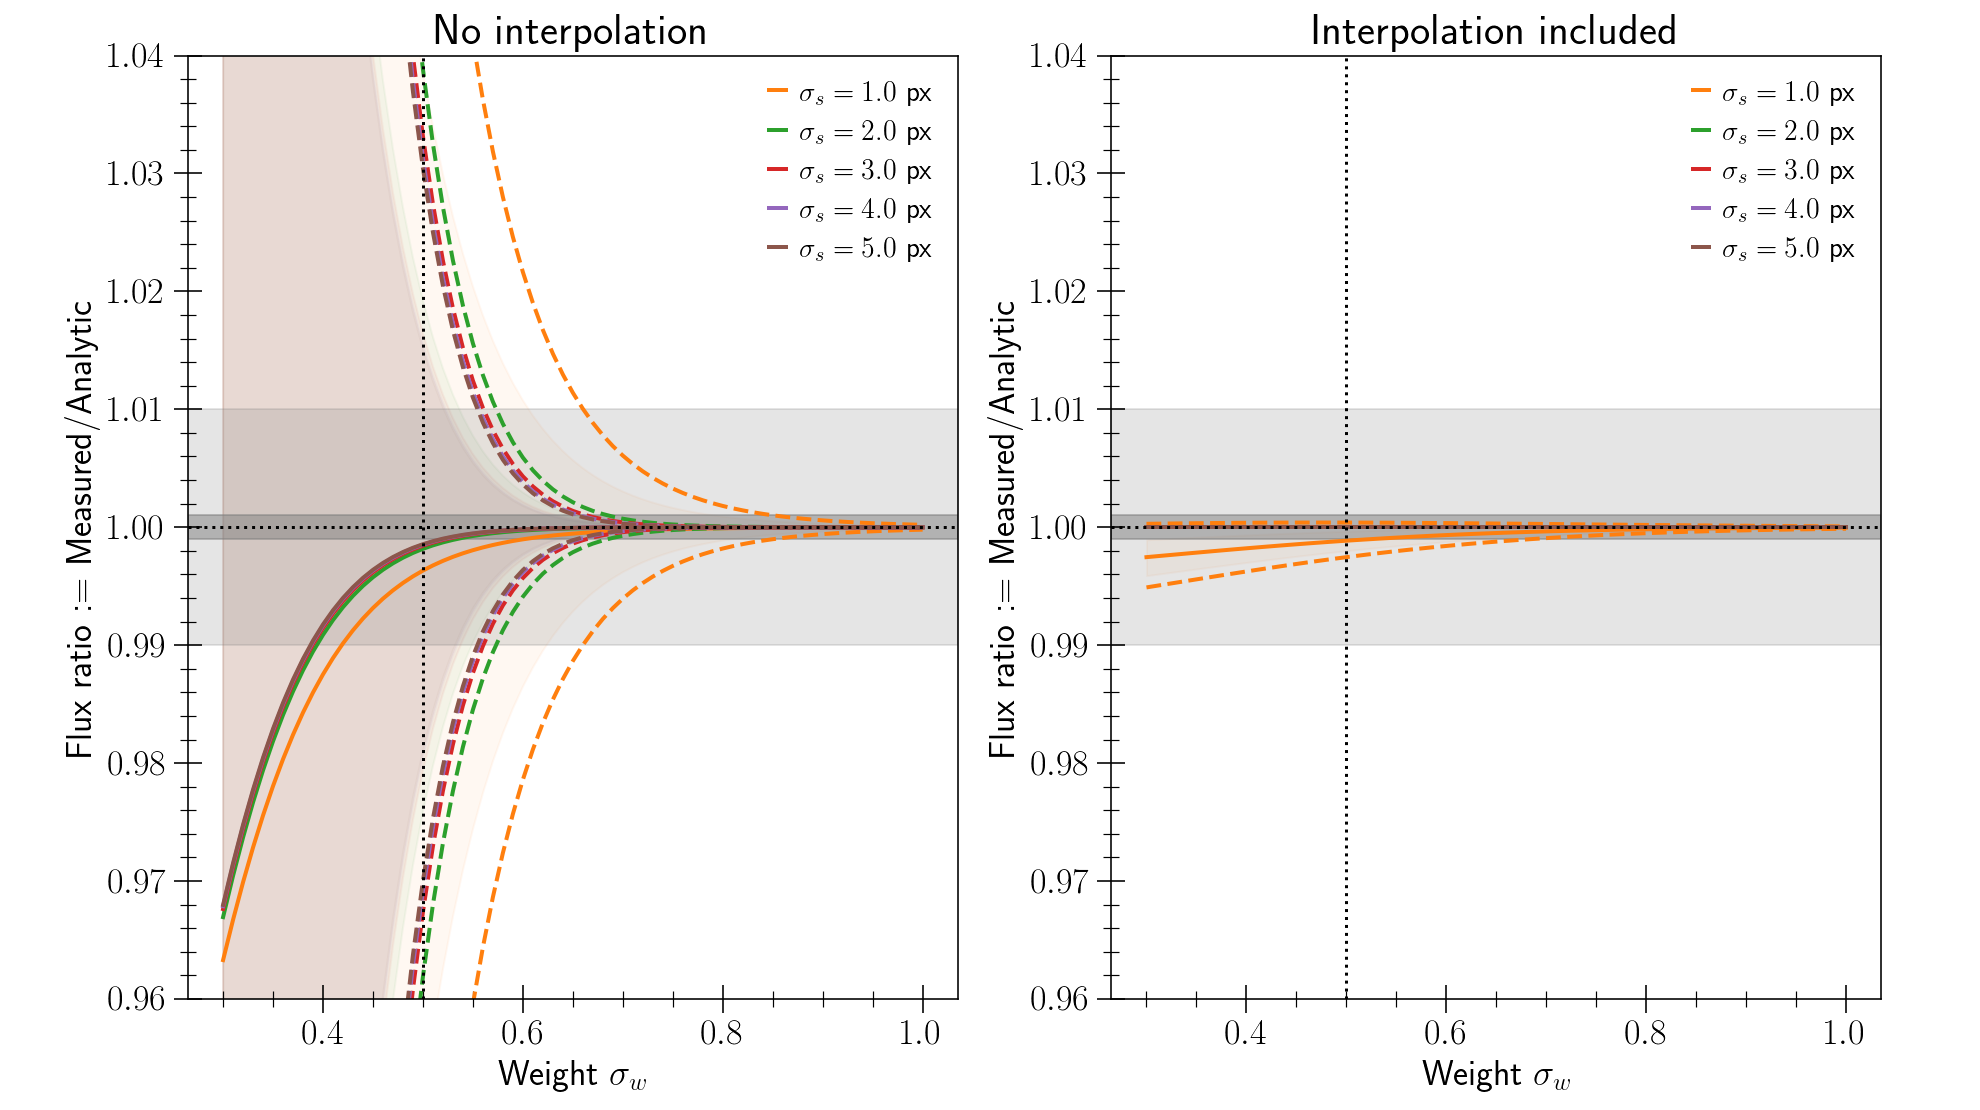
\includegraphics[scale=0.2]{figures/interpolation.png}
    \caption{Plots of the ratio of measured flux to the expectation from analytical expression vs. size of the pre-seeing weight function ($\sigma_w$) for five different source sizes ($\sigma_s$).
    The right panel shows the ratio with the \texttt{sinc} interpolation turned on, and the panel on the left shows without.
    The solid lines show the mean ratio when averaged over all possible sub-pixel offsets.
    The filled regions show the 16-84 percentile region while the dashed lines show the minimum and maximum possible values.
    The dark and the light gray shaded horizontal regions represent 0.1\% and 1\% relative errors in the measured flux, respectively.}
    \label{fig:interpolation}
\end{figure}

The integral in Eq.~\ref{eq:A16} is computed using \texttt{computeFixedMomentsFlux}\footnote{
  Note: \texttt{computeFixedMomentsFlux} computes the flux of an image $I({\bf x})$ weighted by an aperture ${\bf Q}$ as $2\int\rmd{\bf x}\, I({\bf x})\exp\left(-\frac{1}{2} {\bf x}^T {\bf Q}^{-1}{\bf x}\right)$, with a factor 2 in the normalization. This is such that if $I({\bf x})$ is a Gaussian with shape ${\bf Q}$ and has a total flux $F$, the integral evaluates to $F$.}
  by passing the PSF-Gaussianized image and shape parameter $({\bf W}-p^2{\bf 1})$.
This method evaluates the Gaussian weight at pixel centers and computes the inner product with the pixel values of the PSF-Gaussianized image.
For Nyquist-limited samples of band-limited function,
\begin{equation}
    \int\rmd{x}\, f(x) g(x) = \sum_{n} g[n]\, f[n]
\end{equation}

Even though the observed image will be band-limited to some extent, the Gaussian aperture we apply is not.
As a result, the inner product will be biased estimator of the integral.
In particular, the measured flux becomes sensitive to where the centroid is located with a pixel.
In principle, one needs to interpolate the pixels to form a continuous function, and then integrate the function with the Gaussian aperture (see \cite{Bickerton2013}).
However, this procedure is computationally expensive.

%For top-hat apertures, the integral over the image is simply the sum of the pixels, except at the edges that partially overlap the pixels.
%This holds true because the pixel response integrates the light profile within the pixel region.
%However, for a continuously varying aperture such as a Gaussian, it is not obvious if we can sum the product of discretely sampled Gaussian with the image.

To quantify whether we can nevertheless make this approximation, and if so, when this approximation breaks down, the following setup is used.
For simplicity, consider a circular Gaussian source with an effective PSF (includes pixel response) such that the observed profile is a circular Gaussian.
We denote its size (in pixels) as $\sigma_s$ and the size (in pixels) of the circular Gaussian weight function by $\sigma_w$.
The image is rendered with sub-pixel offsets uniformly varying from zero to half a pixel offset in either directions.
The centroid of the Gaussian aperture coincides with the centroid of the source for each of the cases.
The GAaP flux is measured for a range of $\sigma_w$ and $\sigma_s$ values and the results are plotted in the left panel of Fig.~\ref{fig:interpolation}.
For large values of $\sigma_s$ and $\sigma_w$, the measured flux is in agreement with the value expected analytically.
For $\sigma_w \lesssim 0.7$, the measured flux becomes strongly dependent on the sampling locations, even for large values of $\sigma_s$.
After marginalizing over the centroid locations, the mean flux is still an underestimate of the expected value.

If we instead interpolate the pixels with a \texttt{sinc} function to form a continuous function and then evaluate the integral, the measured flux is in much better agreement with the analytical expections.
Adapting the method suggested in~\cite{Bickerton2013} for Gaussian apertures, we compute a set of coefficients to take inner product with the pixel values of the image.
The measured fluxes agree with the expectation for large ($\sigma_s \gtrsim 2$) and biased only slightly for $\sigma_s \sim 1$ when $\sigma_w \lesssim 0.6$

If we measure its flux from pixellated images with a circular Gaussian aperture of size $\sigma_w$ pixels, the expected GAaP flux is $F\left(1+\frac{\sigma_s^2}{\sigma_w^2}\right)^{-1}$ (see Eq.~\ref{eq:gauss_gaap_flux}).
Fig.~\ref{fig:interpolation} shows that with the interpolation turned on, the measured flux is largely insensitive to the sub-pixel offset of the centroid unless both the source and the aperture are narrow, where a small negative bias is seen.
Without the interpolation, a large scatter can be seen for $\sigma_w \lesssim 0.7$ pixels due to the location of the centroid within the central pixel, with the mean marginalized over the centroid location shows a negative bias as well, even for large sources.
\texttt{computeFixedMomentsFlux} turns on the interpolation automatically when $\sigma_w \le 0.5$ pixels.
This will cause the measured flux to change abruptly that may be significant for small sources.

For $\sigma \gtrsim 0.85$ pixels, the flux is accurate to better than 0.1\%.
In practice, we do not expect to use such narrow Gaussian apertures.

\subsection{Estimating noise covariance}
Let us calculate the covariance $C^G$ between the errors on two pixel values $G({\bf x})$ and $G({\bf y})$. Rewriting Eq. A9 of \cite{Kuijken2015}, we get
\begin{equation}
  Cov(G({\bf x}), G({\bf y})) = \int\int\rmd{\bf x}'\rmd{\bf y}'\, Cov(I({\bf x}'),I({\bf y}'))\, K({\bf x}-{\bf x}')K({\bf y}-{\bf y}')
\end{equation}

In KiDS papers, including \cite{Kuijken2015}, translational invariance is assumed and $Cov(I({\bf x}'),I({\bf y}'))$ is expressed as a function of $({\bf x}'-{\bf y}')$ alone and an appropriate covariance matrix is constructed empirically.

However, in Rubin science pipelines, we keep track of the variance (and only variance) per pixel.
So, our model for $Cov(I({\bf x}'), I({\bf y}')) = \sigma^2({\bf x}')\delta_D({\bf x'}-{\bf y}')$, where $\sigma^2({\bf x}')$ is given by the variance plane.
This is an approximation, as the noise \emph{is} correlated on the coadds. However, we proceed with the information we have available. Substituting this in the above equation, we get
\begin{equation}
  Cov(G({\bf x}), G({\bf y})) = \int\rmd{\bf x}'\, \sigma^2({\bf x}') K({\bf x}-{\bf x}')K({\bf y}-{\bf x}')
\end{equation}

The kernel $K$ is expected to be compact, and if the variance plane is slowly varying, we can approximate $\sigma^2({\bf x}')$ by the variance value at the centroid of the source, say $\sigma^2$. This approximation is further justified because of Gaussian weighting we will employ in Eq.~\ref{eq:A17}, which makes the effective kernel even more compact. Redefining ${\bf x}' \rightarrow {\bf x} - {\bf x}'$ ($\rmd{\bf x}' \rightarrow \rmd{\bf x}'$ because the dimensionality is even), we get
\begin{equation}
  Cov(G({\bf x}), G({\bf y})) \approx \sigma^2 \xi_K({\bf r}) \equiv C^G({\bf r}),
\end{equation}
where ${\bf r} = {\bf y}-{\bf x}$. Thus, the covariance is the auto-correlation function of the kernel $K$ $\xi_K({\bf r}) \equiv \int\rmd{\bf x}\, K({\bf x})K({\bf x}+{\bf r})$  scaled by the variance $\sigma^2$ at the location of the source. The auto-correlation function is computed by the \texttt{\_computeKernelAcf} static method.

\subsection{Estimating uncertainties}
Eq. A17 of~\cite{Kuijken2015} says
\begin{equation}
    \text{Var}(F_{\bf W}) = \frac{\det({\bf W})}{\det({\bf W}-p^2\bf{1})} \pi \det({\bf W}-p^2{\bf 1})^{1/2} \int\rmd {\bf x}\, C^G({\bf x}) \exp\left(-\frac{1}{4}{\bf x}^T({\bf W}-p^2{\bf 1})^{-1}{\bf x}\right).
    \label{eq:A17}
\end{equation}
Note the missing factor of $2^{1/2}$, which is an error in \cite{Kuijken2015}.
Since we represent
\begin{equation}
    C^G({\bf r}) = \sigma^2 \xi_{K}({\bf r}),
\end{equation}
we get
\begin{equation}
  \text{Var}(F_{\bf W}) = \frac{\det({\bf W})}{\det({\bf W}-p^2\bf{1})}\left(\frac{1}{2}\right)^2 \times 4\pi \sigma^2 \det({\bf W}-p^2{\bf 1})^{1/2} \times \int\rmd {\bf r}\, \xi_{K}({\bf r}) \exp\left(-\frac{1}{2}{\bf r}^T(2({\bf W}-p^2{\bf 1}))^{-1}{\bf r}\right).
\end{equation}
We categorize them into three terms, separated by $\times$.
\begin{enumerate}
  \item The naive calculation of flux variance by \texttt{computeFixedMomentsFlux} yields the middle term $4\pi \sigma^2 \det({\bf W}-p^2{\bf 1})^{1/2}$ (given by \texttt{instFluxErr}$^2$).
  \item The factor $\frac{1}{4}\frac{\det({\bf W})}{\det({\bf W}-p^2\bf{1})}$ appears because of the scaling factor in $F_{\bf W}$ (Eq. A16 of \cite{Kuijken2015}).
  \item The square root of the integral is computed by \texttt{\_getFluxErrScaling} and referred to as \texttt{fluxErrScaling}. This is the actual contribution due to correlations in the noise introduced by PSF-Gaussianization procedure. This is computed using \texttt{computeFixedMomentsFlux} on the auto-correlation function, with $2 \times$ the shape parameter of aperture used to measure $F_{\bf W}$.

  If the PSF had been Gaussian to begin with, or if we were neglecting the effects of correlated noise on flux uncertainties, $K({\bf r}) = \delta_D({\bf r})$. This leads to the integral evaluating to 1.
\end{enumerate}

\subsubsection{Alternative representation}
Note that from the definition of $\xi_K({\bf r})$, it follows that
\begin{align}
  \int\rmd{\bf r}\, \xi_K({\bf r}) &= \int\rmd{\bf r}\, \int\rmd{\bf x}\, K({\bf x})K({\bf x}+{\bf r})\\
                                   &= \int\rmd{\bf x}\, K({\bf x}) \int\rmd{\bf r}\, K({\bf x}+{\bf r})\\
                                   &= \left[ \int\rmd{\bf x}\, K({\bf x})\right]^2
                                   \label{eq:integral_acf}
\end{align}

In a similar manner, the integral for \texttt{fluxErrScaling} can also be expressed as
\begin{equation}
  \int\rmd {\bf r}\, \xi_{K}({\bf r}) \exp\left(-\frac{1}{2}{\bf r}^T(2({\bf W}-p^2{\bf 1}))^{-1}{\bf r}\right) =
  \left[ \int\rmd{\bf x}\int\rmd{\bf y} K({\bf x}-{\bf y}) \exp\left(-\frac{1}{2}{\bf y}^T({\bf W}-p^2{\bf 1})^{-1}{\bf y}\right)\right]^2.
\end{equation}
The proof follows by considering $\int\rmd{\bf x} f({\bf x}) = \tilde{f}(0)$, where $\tilde{f}$ is the Fourier transform of $f$.

\section{Concluding remarks}
This technote presents the Gaussian Aperture and PSF photometry algorithm and covers various technical details with regards to its implementation in the Rubin Science Pipelines.
This note also captures various calculations that are used in testing the code, since they are cumbersome to leave as comments within the code itself.

\appendix
% Include all the relevant bib files.
% https://lsst-texmf.lsst.io/lsstdoc.html#bibliographies
\section{References} \label{sec:bib}
\renewcommand{\refname}{} % Suppress default Bibliography section
\bibliography{local,lsst,lsst-dm,refs_ads,refs,books}

% Make sure lsst-texmf/bin/generateAcronyms.py is in your path
\section{Acronyms} \label{sec:acronyms}
\addtocounter{table}{-1}
\begin{longtable}{p{0.145\textwidth}p{0.8\textwidth}}\hline
\textbf{Acronym} & \textbf{Description}  \\\hline

DM & Data Management \\\hline
DMTN & DM Technical Note \\\hline
GAaP & Gaussian-Aperture and PSF photometry \\\hline
KiDS & Kilo-Degree Survey \\\hline
PSF & Point Spread Function \\\hline
\end{longtable}

% If you want glossary uncomment below -- comment out the two lines above
%\printglossaries

\begin{comment}
\section{Consistent colors}
We model the intrinsic galaxy
\begin{equation}
  g({\bf x}; \lambda) \approx \sum_{c=b,d} A_c c({\bf x}; M_c) S_c(\lambda; z),
\end{equation}
where $A_c, M_c$ can vary from one galaxy to another. $S_c(\lambda, z) = S_c((1+z)^{-1}\lambda; 0)$.
The image of the galaxy seen through a band $k$ is
\begin{equation}
  g_k({\bf x}) = \int\mathrm{d}\lambda f_k(\lambda) g({\bf x}; \lambda)
\end{equation}

The fluxes
\begin{equation}
  F_k = \int\rmd{\bf x} g_k({\bf x}) = \sum_{c=b,d}A_c \int\rmd{\bf x}  A({\bf x})c({\bf x}; M_c)\int\mathrm{d}\lambda f_k(\lambda)S_c(\lambda; z)
\end{equation}

This can be generalized to arbitrary number of components, until each component represents a star: $c({\bf x}; M_c) = \delta_D({\bf x}-{\bf x}_c)$.

The choice of the aperture function $A({\bf x})$ affects only the irrelevant linear combination coefficient, which is a free parameter. It therefore amounts to a redefinition of the coefficient. The information about the redshift is preserved.

Given a set of galaxy fluxes in different bands $\{ F_k \}_k$, a template based Bayesian redshift code estimates a point redshift, or a posterior distribution for redshift $p(z)$ by constructing a model $\sum_t a_t t({\bf x}; M_t) S_t(\lambda; z)$
\end{comment}

\section{Gaussian integrals}
The integrals in computing various GAaP quantities can be computed analytically when the PSF and the intrinsic sources are Gaussian.
We will derive the analytical results that are used in the unit testing of the code.

For an intrinsic Gaussian source $g({\bf x})$ of total flux $F$ and shape ${\bf S}$ and a Gaussian aperture of shape ${\bf W}$,
it follows from the definition \ref{eq:A16} that its GAaP flux is
\begin{align}
  F_{\bf W} &= \int\rmd{\bf x}\, \left[\frac{F}{2\pi\det({\bf S})} \exp\left( -\frac{1}{2}{\bf x}^T{\bf S}^{-1}{\bf x} \right)\right] \exp\left( -\frac{1}{2}{\bf x}^T{\bf W}^{-1}{\bf x} \right) \\
            &= \frac{F}{2\pi\det({\bf S})}\int\rmd{\bf x}\, \exp\left(-\frac{1}{2}{\bf x}^T({\bf S}^{-1}+{\bf W}^{-1}) {\bf x}\right) \\
            &= F\frac{2\pi\det\left({({\bf S}^{-1}+{\bf W}^{-1})}^{-1}\right)}{2\pi\det({\bf S})} \\
            &= F\frac{1}{\det({\bf S})\det({\bf S}^{-1}+{\bf W}^{-1})} \\
            &= F\frac{\det({\bf S}^{-1})}{\det({\bf S}^{-1}+{\bf W}^{-1})} \text{ (or) }\frac{F}{\det({\bf 1} + {\bf S W}^{-1})}.
  \label{eq:gauss_gaap_flux}
\end{align}
If ${\bf S} = \sigma_s^2{\bf 1}$ and ${\bf W} = \sigma_w^2{\bf 1}$, then $F_{\bf W} = F\left(1+\frac{\sigma_s^2}{\sigma_w^2}\right)^{-1}$.

Suppose $I({\bf x})$ has a circular Gaussian PSF of size $s$ and the target PSF is a Gaussian PSF of size $p = fs$ ($f>1$), then the kernel $K$ is also a Gaussian of size $s(f^2-1)^{1/2}$.
In the GAaP plugin, the values for $f$ are given by \texttt{scalingFactors}.

Since flux-conservation implies $\int\rmd{\bf x}\, K({\bf x}) = 1$, we can immediately write
\begin{equation}
  K({\bf x}) = \frac{1}{2\pi (f^2-1)s^2} \exp\left(-\frac{{\bf x}^T{\bf x}}{2(f^2-1)s^2}\right)
\end{equation}

The auto-correlation function $\xi_K({\bf r})$ is then given by
\begin{equation}
  \xi_K({\bf r}) = \frac{1}{4\pi(f^2-1)s^2}\exp\left(-\frac{{\bf r}^T{\bf r}}{4(f^2-1)s^2}\right).
\end{equation}
This is easy to see by first recognizing that $\xi_K({\bf r})$ must be a Gaussian with size $\sqrt{2}$ times larger than that of $K$ and the normalization factor follows that $\xi_K({\bf r})$ must integrate to 1 if $K$ integrates to 1 (see Eq.~\ref{eq:integral_acf}).

The square of the \texttt{fluxErrScaling} parameter is then given by the Gaussian integral
\begin{equation*}
  \int\rmd{\bf r}\,\xi_K({\bf r})\exp(-\frac{{\bf r}^T{\bf r}}{4(\sigma^2-p^2)}),
\end{equation*}
where $\sigma$ is the size of the Gaussian aperture for the pre-seeing source $g({\bf x})$. In the GAaP plugin, these values are given by \texttt{sigmas} config parameter.

The exponents of the Gaussians is simplified as follows.
\begin{equation}
  \frac{{-\bf r}^T{\bf r}}{4}\left(\frac{1}{(f^2-1)s^2} + \frac{1}{(\sigma^2-f^2s^2)} \right)
  = \frac{{-\bf r}^T{\bf r}}{4}\left( \frac{\sigma^2 - s^2}{s^2(f^2-1)(\sigma^2-f^2s^2)} \right)
\end{equation},
where $p$ is replaced by $fs$. Evaluating the Gaussian integral, we get
\begin{align}
  \texttt{fluxErrScaling}^2 &= \frac{1}{4\pi (f^2-1)s^2} \times \frac{\pi 4s^2(f^2-1)(\sigma^2-f^2s^2)}{\sigma^2-s^2} \\
  &= \frac{\sigma^2-f^2s^2}{\sigma^2-s^2}
\end{align}
As a consistency check, we get $\texttt{fluxErrScaling} = 1$ for $f=1$, i.e., if we do not carry out the PSF-Gaussianization procedure. For $f>1$, $\texttt{fluxErrScaling} < 1$. As an aside, if $\xi_K({\bf r}) \ge 0$ for all ${\bf r}$ (as in the Gaussian kernel case), \texttt{fluxErrScaling} is guaranteed to be less than 1. In other words, the naive flux uncertainty overestimates the true uncertainty. For naive errors to be an underestimation of true errors, it is necessary that the kernel should be negative for sufficiently small $|{\bf r}|$. Intuitively, this makes sense; non-negative valued kernel smoothes the noise in the image, reducing its power, whereas as kernel with both positive and negative values has the potential to amplify the random fluctuations in different pixels.

\end{document}
